132. \begin{figure}[ht!]
\center{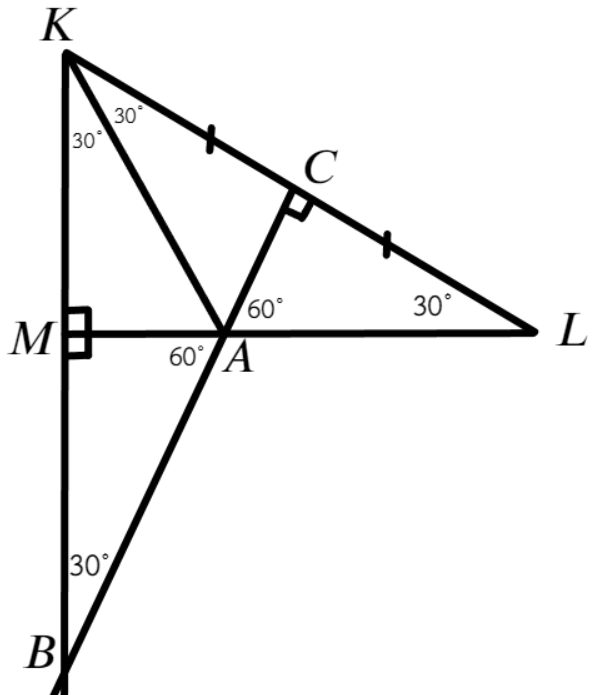
\includegraphics[scale=0.35]{g7-132.png}}
\end{figure}\\
Пусть $C$ --- середина $KL,$ тогда в треугольнике $AKL$ медиана $AC$ совпадает с высотой, значит он равнобедренный и  $AK=AL, \angle AKL=\angle L=30^\circ,$ тогда $\angle MKA=60^\circ-30^\circ=30^\circ,$ а также $\angle CAl=90^\circ-30^\circ=60^\circ,\ \angle MAB=\angle CAL=60^\circ,\ \angle MBA=90^\circ-60^\circ=30^\circ.$
Пусть $AM=x,$ тогда по теореме о катете, лежащем напротив угла в $30^\circ,$ получим $AB=2x,\ AK=2x,\ AL=AK=2x=AB=3$см.\\
